% Advances in Mathematics: Scientific Journal 9 (2020), no.10, 7859–7864
% ISSN: 1857-8365 (printed); 1857-8438 (electronic)
% https://doi.org/10.37418/amsj.9.10.18
% Special Issue on ACMAMP‑2020

\documentclass[11pt]{amsart}

% -----------------------------------------------------------------------------
%     Packages
% -----------------------------------------------------------------------------
\usepackage{amsmath,amssymb,amsfonts,amsthm}
\usepackage{url}
\usepackage{geometry}
\usepackage{hyperref}
\usepackage[backend=biber, style=numeric, sorting=none, defernumbers=true, doi=true, url=true]{biblatex}
\usepackage{mathrsfs}
\usepackage{fullpage}
\usepackage{setspace}
\usepackage{graphicx}
\usepackage{float}
\usepackage{caption}
\usepackage{subcaption}
\usepackage{booktabs}
\usepackage{doi}

% -----------------------------------------------------------------------------
%     Geometry & Hyperref setup
% -----------------------------------------------------------------------------
\addbibresource{references.bib}
\geometry{
  paper=a4paper,
  total={160mm,247mm},
  left=25mm,
  top=25mm,
}
\hypersetup{
  colorlinks=true,
  linkcolor=black,
  citecolor=black,
  urlcolor=black,
  pdftitle={Mathematical Signatures of Malignancy: Forecasting Glioblastoma Multiforme By Implementing Graph Algorithms in Gene Coexpression Networks},
  pdfauthor={Adityakrishna SreeRamachandrarao and Anusha Lakshmi Dharmavathi and Satyavathi Dronamraju},
}

% -----------------------------------------------------------------------------
%     Theorem styles (AMSJ house‑style)
% -----------------------------------------------------------------------------
\theoremstyle{plain}
\newtheorem{theorem}{Theorem}[section]
\newtheorem{proposition}[theorem]{Proposition}
\newtheorem{lemma}[theorem]{Lemma}
\newtheorem{corollary}[theorem]{Corollary}
\theoremstyle{definition}
\newtheorem{definition}[theorem]{Definition}
\theoremstyle{remark}
\newtheorem*{remark}{Remark}

% -----------------------------------------------------------------------------
%     Shortcuts
% -----------------------------------------------------------------------------
\newcommand{\Z}{\mathbb{Z}}
\newcommand{\N}{\mathbb{N}}
\newcommand{\set}[1]{\left\{#1\right\}}
\newcommand{\abs}[1]{\left\lvert #1 \right\rvert}

% -----------------------------------------------------------------------------
%     Front‑matter
% -----------------------------------------------------------------------------
\title[A Computational Biomedical Oncology Approach to Glioblastoma Multiforme: Graph-Theoretic Signatures in Gene Coexpression Networks]{A Computational Biomedical Oncology Approach to Glioblastoma Multiforme: Graph-Theoretic Signatures in Gene Coexpression Networks}

\author{
Adityakrishna SreeRamachandrarao\textsuperscript{1} \and
Anusha Lakshmi Dharmavathi\textsuperscript{2} \and
Satyavathi Dronamraju\textsuperscript{3}
}
\address{Department of Science and Technology, Scientific Researchers LLC, Indianapolis, Indiana, USA}
\email{\textsuperscript{1}asreera110@scientificresearchers.org \and
\textsuperscript{2}anushadronamraju20@scientificresearchers.org \and 
\textsuperscript{3}satyadronamraju11@scientificresearchers.org}

\thanks{\noindent\textsuperscript{1}\,Corresponding author}

\subjclass[2010]{05C69}
\keywords{Gene coexpression, Pearson's Correlation Coefficient, Mann-Whitney U test}


\begin{document}

\bigskip

% -----------------------------------------------------------------------------
%     Abstract
% -----------------------------------------------------------------------------
\begin{abstract}
Conventional genomic analyses of cancer focus on individual high-risk mutations, yet many malignancies arise in their absence, underscoring the need for a more holistic screening paradigm. We propose graph theory as such a framework: genes are modeled as nodes, statistically significant coexpression relationships (Pearson's correlation with $p\text{-value} < 0.05$, Benjamini--Hochberg corrected) as weighted edges, and the resulting gene coexpression network encodes collective regulatory behavior invisible to single-gene methods. Using glioblastoma multiforme (GBM) and normal brain expression data from TCGA and GTEx respectively, we identify four mathematical signatures that distinguish cancer from normal networks: (i) degree distribution and power-law exponent, (ii) clique cover number and Ramsey substructure, (iii) $k$-core decomposition, and (iv) signed Laplacian eigenvalue spectrum. Each signature was tested for statistical significance via the Mann--Whitney $U$ test and bootstrapped goodness-of-fit procedures. Our results confirm significant topological differences across all four metrics, consistent with GBM manifesting as a network-level disorder rather than a collection of isolated mutations. These signatures lay the groundwork for a graph-theoretic biomarker framework applicable to early cancer detection and, prospectively, to a meta-analysis spanning multiple cancer types.
\end{abstract}

\maketitle

% -----------------------------------------------------------------------------
%     Section 1: Introduction
% -----------------------------------------------------------------------------
\section{Introduction}
Glioblastoma multiforme (GBM) is the most aggressive form of astrocytic tumor, characterized by rapid proliferation, extensive infiltration, and poor response to therapy. Despite decades of sequencing efforts, median patient survival after diagnosis remains under 15 months, and targeted single-gene therapies have achieved only modest gains \cite{jeong2001lethality}. This persistent failure highlights a fundamental limitation of reductionist approaches: cancer is not simply the consequence of one or two mutant genes, but an emergent phenomenon arising from dysregulated interactions across entire gene regulatory networks.

Graph theory provides a natural mathematical language for capturing such network-level phenomena. Representing genes as nodes and coexpression relationships as edges transforms a high-dimensional transcriptomic dataset into a topological object whose global properties can be analyzed with precision. Differences between healthy and malignant tissue can then be framed as differences in network topology---differences that may be quantified, tested statistically, and used as predictive signatures of malignancy.

This paper investigates whether GBM leaves reproducible mathematical signatures in gene coexpression networks and whether such signatures can be rigorously characterized using tools from graph theory and spectral analysis. We identify four such signatures, derive the mathematical foundations underpinning each, and validate their discriminatory power against GBM and normal brain expression data.

% -----------------------------------------------------------------------------
%     Section 2: Application of Graph Networks
% -----------------------------------------------------------------------------
\section{Application of Graph Networks}
Mathematical and computational models are increasingly indispensable in biomedical research, where in vivo and in vitro studies face both scientific and ethical constraints. In this study, all analyses were conducted in silico using glioblastoma multiforme and normal brain gene expression data. After systematic investigation, four graph-theoretic signatures were identified as particularly informative for distinguishing cancer from normal gene coexpression networks. Each captures a distinct structural property of the network, and together they provide a multidimensional characterization of malignancy.

The first signature is degree distribution and power-law exponent. We hypothesize that cancer networks exhibit scale-free behavior more pronounced than in normal networks. Scale-free networks are characterized by a power-law degree distribution \cite{barabasi1999emergence} and preferential attachment dynamics, in which highly connected hub nodes accumulate additional connections at a disproportionate rate \cite{newman2005power}. In the oncogenic context, hub regulatory genes become overexpressed, driving unchecked cellular proliferation in a positive feedback loop \cite{jeong2001lethality}. As a consequence, the power-law exponent $\gamma$ is expected to be lower in cancer networks, reflecting heavier degree tails and greater hub dominance \cite{barabasi1999emergence}.

The second signature is clique cover number and Ramsey substructure. The clique cover number quantifies how many complete subgraphs are required to cover all vertices of a graph \cite{golumbic2004algorithmic}. Ramsey theory guarantees that in any sufficiently large graph, large cliques or independent sets must appear \cite{graham1990ramsey}, and furthermore that predictable dense substructures will emerge \cite{erdos1935combinatorial}. We hypothesize that cancer networks exhibit higher clique cover numbers, reflecting aberrant interconnectivity arising from metabolic rewiring and immune evasion. Integrating Ramsey theory, we further predict that the relationship between clique density and clique size will reveal a distinctive substructure in the cancer network that is absent in the normal network.

The third signature is $k$-core decomposition. The $k$-core of a graph is the maximal subgraph in which every vertex has degree at least $k$, and iterative peeling reveals a hierarchical organization of central versus peripheral nodes \cite{seidman1983network,batagelj2003core}. Deep $k$-cores identify sets of genes that are densely and mutually co-regulated, which has proven informative in protein interaction networks \cite{wuchty2003evolutionary}. We hypothesize that cancer networks harbor deeper $k$-cores corresponding to tightly reinforced oncogenic modules, even as peripheral connectivity becomes more fragmented due to mutation-induced edge loss and sparse network rewiring. This produces a characteristic co-existence of a dense inner shell and a disrupted periphery that is not observed in normal networks.

The fourth and final signature is the signed Laplacian eigenvalue spectrum. The signed Laplacian is constructed from the difference between the signed degree matrix and the signed adjacency matrix, and accommodates the negative-weight edges that arise from inhibitory coexpression relationships \cite{kunegis2010spectral}. The second-smallest eigenvalue, the algebraic connectivity, measures global cohesion and robustness \cite{fiedler1973algebraic}. The multiplicity of the zero eigenvalue gives the number of balanced connected components, while negative eigenvalues indicate structurally unbalanced cycles arising from antagonistic regulatory modules \cite{hou2005bounds}. Higher-order spectral moments reflect pathway redundancy \cite{chung1997spectral}. We hypothesize that cancer networks will exhibit lower algebraic connectivity, more negative eigenvalues, and a broader eigenvalue spectrum than normal networks, all consistent with the fractured, conflicting regulatory architecture of malignant tissue.

Table~\ref{tab:hypotheses} summarizes the hypothesized differences between cancer and normal networks for each signature.

{\Large
\begin{table}[H]
\centering
\caption{Comparison of Hypothesized Graph Features}
\label{tab:hypotheses}
\renewcommand{\arraystretch}{1.8}
\resizebox{\textwidth}{!}{
\begin{tabular}{@{}llll@{}}
\toprule
\textbf{Metric} & \textbf{Cancer Network (Glioblastoma)} & \textbf{Normal Brain Network} \\
\hline
\textbf{Degree Distribution \& Power-Law} & Heavier tail; lower $\gamma$ ($\gamma \approx 2.0$--$2.5$); more hubs & Lighter tail; higher $\gamma$ ($\gamma \approx 2.5$--$3.5$); fewer hubs \\
\hline
\textbf{Clique Cover \& Ramsey Structure} & Higher clique cover; overlapping, conflicting communities & Lower clique cover; modular but cleaner community boundaries \\
\hline
\textbf{k-Core Decomposition} & Higher max coreness; deeper, tightly nested cores & Lower coreness; flatter, less nested hierarchy \\
\hline
\textbf{Laplacian (or Signed) Spectrum} & Spread out, with possible \textbf{negative} eigenvalues (due to dysregulation) & Tightly clustered, all positive eigenvalues; highly cohesive \\
\bottomrule
\end{tabular}
}
\end{table}
}

% -----------------------------------------------------------------------------
%     Section 3: Materials and Methods
% -----------------------------------------------------------------------------
\section{Materials and Methods}
Gene expression data were obtained from two public repositories: TCGA (The Cancer Genome Atlas) \cite{gbmcancerdata} for GBM tumor samples, and GTEx (Genotype-Tissue Expression) \cite{normalbraindata} for matched normal brain samples. This pairing enables a controlled comparative analysis between malignant and healthy transcriptomes.

Network construction was performed in Python using the NetworkX library. A random subset of genes was selected from the cancer dataset, and the corresponding genes were identified in the normal dataset. After filtering lowly expressed genes and applying a $\log_2$ transformation to stabilize variance, Pearson's correlation coefficients were computed for every pairwise gene combination. A correlation was included as a network edge only if the associated $p$-value satisfied $p < 0.05$, and multiple testing was controlled using the Benjamini--Hochberg false discovery rate procedure \cite{benjaminihochberg1995}. Outlier samples were excluded prior to network construction to prevent spurious correlations. The resulting signed, weighted gene coexpression networks---one for GBM and one for normal brain---were then subjected to the four graph-theoretic analyses described below.

\subsection{Degree Distribution in Networks}
The degree of a node $i$, denoted $k_i$, is the number of edges incident on that node. The degree distribution $P(k)$ is the probability that a randomly selected node has degree exactly $k$. In many real-world networks, the tail of $P(k)$ follows a power law:
\[
  P(k) \sim C\,k^{-\alpha}, \quad k \ge k_{\min},
\]
where $\alpha>1$ is the power-law exponent, $k_{\min}$ is the lower cutoff above which the power law holds, and $C$ is a normalization constant:
\[
  C = \biggl(\sum_{k=k_{\min}}^{\infty} k^{-\alpha}\biggr)^{-1}.
\]

\subsection{Maximum-Likelihood Estimation of \texorpdfstring{$\alpha$}{alpha}}
Given observed degrees $\{k_i\}$ with $k_i \ge k_{\min}$ for $i=1,\dots,n$, the maximum-likelihood estimator (MLE) of $\alpha$ for discrete data is \cite{clauset2009power}:
\[
  \widehat{\alpha}
  = 1 + n \biggl[ \sum_{i=1}^n \ln\!\Bigl(\frac{k_i}{k_{\min} - 0.5}\Bigr) \biggr]^{-1}.
\]
This estimator minimizes the negative log-likelihood
\[
  \mathcal{L}(\alpha) = -\,n\ln C(\alpha,k_{\min}) + \alpha \sum_{i=1}^n \ln k_i.
\]
The lower cutoff $k_{\min}$ is selected by minimizing the Kolmogorov--Smirnov (KS) distance between the empirical cumulative distribution function (CDF) and the fitted power-law CDF.

\subsection{Goodness-of-Fit \texorpdfstring{$p$}{p}-Value via Bootstrapping}
To test whether a power law is a plausible model for the observed degree sequence:
\begin{enumerate}
  \item Fit $\widehat{\alpha}$ and record the KS statistic $D_{\rm obs}$.
  \item Generate many synthetic datasets of size $n$ drawn from a power law with exponent $\widehat{\alpha}$ and the same $k_{\min}$.
  \item Refit each synthetic dataset to obtain its KS statistic $D_{\rm synth}$.
  \item The $p$-value is the fraction of synthetic statistics that exceed the observed value:
    \[
      p = \frac{\#\{D_{\rm synth} \ge D_{\rm obs}\}}{\text{number of simulations}}.
    \]
  If $p>0.1$, the power-law model is considered plausible; if $p<0.1$, it is rejected.
\end{enumerate}

\subsection{Log-Likelihood Ratio Tests}
To compare the power-law model against an alternative heavy-tailed distribution, consider two competing probability mass functions $p_1(k)$ and $p_2(k)$. Their log-likelihoods on the observed data $\{k_i\}$ are
\[
  \mathcal{L}_1 = \sum_{i=1}^n \ln p_1(k_i), \quad
  \mathcal{L}_2 = \sum_{i=1}^n \ln p_2(k_i).
\]
The log-likelihood ratio is
\[
  R = \mathcal{L}_1 - \mathcal{L}_2.
\]
A positive $R$ indicates support for model~1 (e.g., power law over exponential), while $R<0$ favors model~2. Statistical significance is assessed using Vuong's method \cite{Vuong1989}.

\subsection{Clique Cover Number}
For a graph $G=(V,E)$, a \emph{clique cover} is a collection of cliques $\{C_1,\dots,C_k\}$ such that every vertex $v\in V$ lies in at least one $C_i$. The \textbf{clique cover number} $\theta(G)$ is the minimum number of cliques in such a collection:
\[
  \theta(G)
  = \min\bigl\{k : \exists\, C_1,\dots,C_k \text{ all cliques, } V = \textstyle\bigcup_{i=1}^k C_i \bigr\}.
\]
Covering $V$ by cliques in $G$ is equivalent to coloring the complement graph $\overline{G}$, so
\[
  \theta(G) = \chi\bigl(\overline{G}\bigr),
\]
where $\chi$ denotes the chromatic number. If $\omega(G)$ denotes the maximum clique size in $G$, then
\[
  \omega(G) \le\, \theta(G) \le\, |V|.
\]

\subsection{Ramsey Theory}
The \emph{Ramsey number} $R(s,t)$ is the smallest integer $N$ such that every graph on $N$ vertices contains either a clique of size $s$ or an independent set of size $t$:
\[
  R(s,t) = \min\{N : \forall\,G\text{ on }N\text{ vertices, } \omega(G)\ge s \;\vee\; \alpha(G)\ge t\}.
\]
Erd\H{o}s and Szekeres proved the classical bound:
\[
  R(s,t) \le \binom{s+t-2}{s-1},
  \quad\text{and in particular}\quad
  R(s,s) \le \binom{2s-2}{s-1} \sim \frac{4^{s-1}}{\sqrt{\pi(s-1)}}.
\]

\subsection{K-core Decomposition}
Let $G = (V,E)$ be an undirected graph. The \emph{$k$-core} of $G$ is the maximal subgraph in which every vertex has degree at least $k$:
\[
C_k(G)
\;=\;
\max \bigl\{\,H = (V_H, E_H)\subseteq G : \delta(H)\ge k\bigr\},
\]
where $\delta(H)$ denotes the minimum degree of subgraph $H$. Each node $v\in V$ is assigned a \emph{core number}
\[
\phi(v)
\;=\;
\max\bigl\{\,k : v\in C_k(G)\bigr\},
\]
which is the largest $k$ such that $v$ survives iterative pruning of all nodes with degree less than $k$.

\subsection{Signed Graph and Laplacian: Theory and Definitions}
Let $G = (V, E^+, E^-)$ be a signed graph, where $E^+$ contains positive (activating) edges and $E^-$ contains negative (inhibitory) edges. The \emph{signed adjacency matrix} $A^s \in \mathbb{R}^{n \times n}$ is defined by
\[
A^s_{ij}
\;=\;
\begin{cases}
+1, & (i,j)\in E^+,\\[4pt]
-1, & (i,j)\in E^-,\\[4pt]
0,  & \text{otherwise}.
\end{cases}
\]
The \emph{signed degree matrix} $D^s$ is diagonal with entries
\[
D^s_{ii}
\;=\;
\sum_{j=1}^n \bigl|A^s_{ij}\bigr|,
\]
counting the total absolute edge weight incident on node $i$. The \emph{signed Laplacian} is
\[
L^s
\;=\;
D^s \;-\; A^s,
\]
which is symmetric and positive semi-definite for structurally balanced graphs. The eigenvalues of $L^s$,
\[
0 \;=\; \lambda_1 \;\leq\; \lambda_2 \;\leq\; \cdots \;\leq\; \lambda_n,
\]
encode the structural balance of the signed graph. The multiplicity of $\lambda = 0$ equals the number of balanced connected components, and the second-smallest eigenvalue $\lambda_2$ (the Fiedler value or algebraic connectivity) measures global network cohesion. The presence of negative eigenvalues in the unsigned Laplacian setting signals structurally unbalanced cycles consistent with antagonistic regulatory interactions.

%%%%%%%%%%%%%%%%%%%%%%%%%%%%%%%%%%%

% -----------------------------------------------------------------------------
%     Section 4: Results and Conclusion
% -----------------------------------------------------------------------------
\section{Results and Conclusion}

\begin{figure}[htbp]
    \centering
    \begin{subfigure}{0.45\textwidth}
        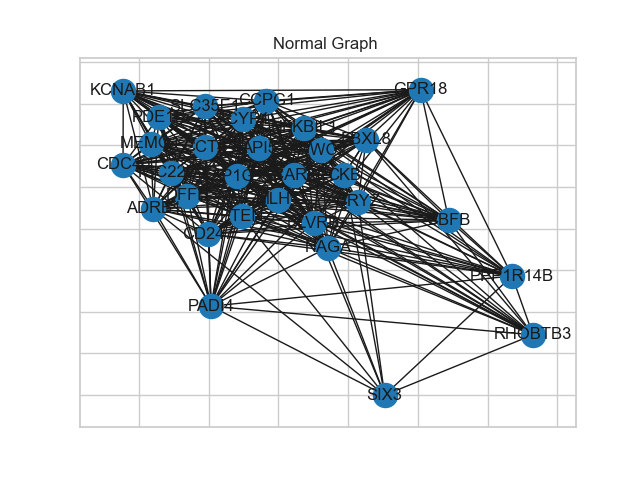
\includegraphics[width=\linewidth]{trial_1_example/trial1norm_net.png}
        \caption{Normal Network}
        \label{fig:graph1}
    \end{subfigure}\hfill
    \begin{subfigure}{0.45\textwidth}
        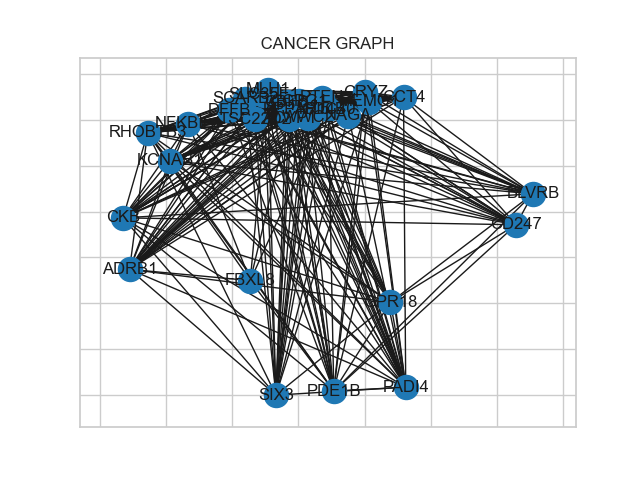
\includegraphics[width=\linewidth]{trial_1_example/trial1onc_net.png}
        \caption{Cancer Network}
        \label{fig:graph2}
    \end{subfigure}
    \caption{Comparison between the normal and GBM gene coexpression networks.}
    \label{fig:graphs}
\end{figure}

\begin{figure}[htbp]
    \centering
    \begin{subfigure}{0.45\textwidth}
        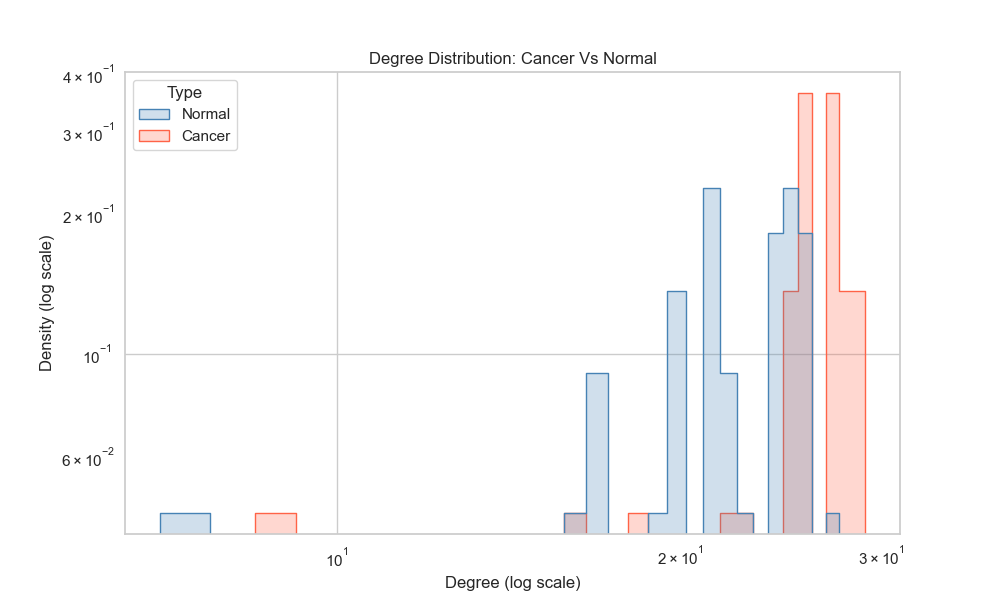
\includegraphics[width=\linewidth]{trial_1_example/trial1powerlaw_comp.png}
        \caption{Degree Distribution and Power Law}
    \end{subfigure}
    \begin{subfigure}{0.45\textwidth}
        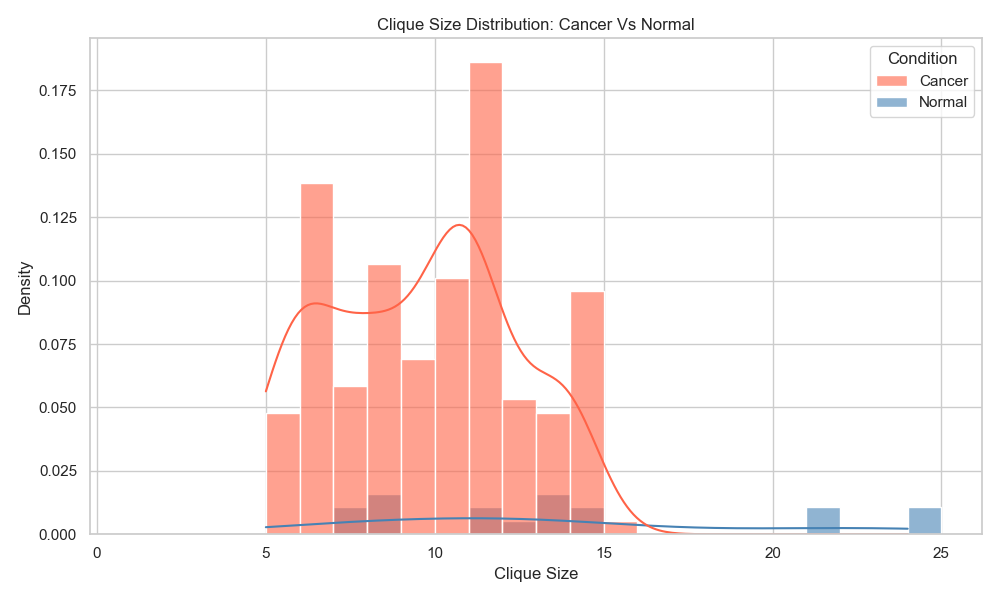
\includegraphics[width=\linewidth]{trial_1_example/trial1cliq_comp.png}
        \caption{Clique Cover Number and Ramsey Theory}
    \end{subfigure}
    \vspace{1em}
    \begin{subfigure}{0.45\textwidth}
        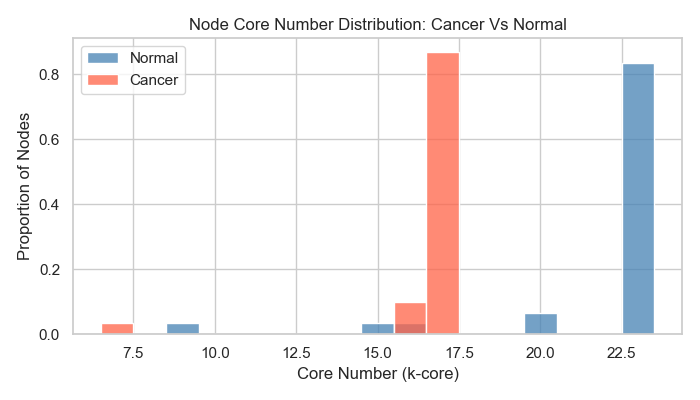
\includegraphics[width=\linewidth]{trial_1_example/trial1k_core_dist.png}
        \caption{K-core Decomposition}
    \end{subfigure}
    \begin{subfigure}{0.45\textwidth}
        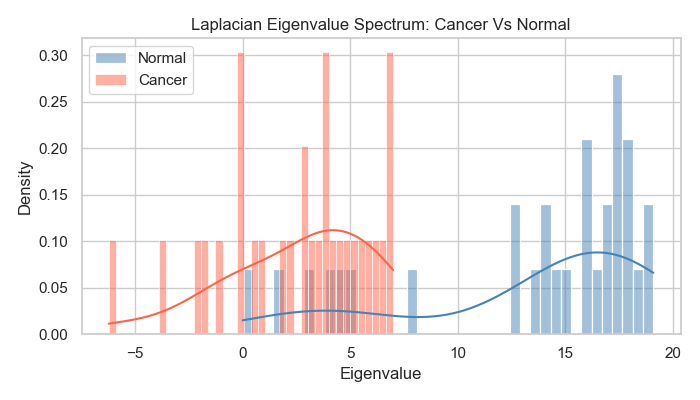
\includegraphics[width=\linewidth]{trial_1_example/trial1laplacian_eigval_spec.png}
        \caption{Laplacian Eigenvalue Spectrum}
    \end{subfigure}
    \caption{Four mathematical signatures of malignancy in GBM versus normal brain coexpression networks.}
    \label{fig:fourimages}
\end{figure}

\subsection{Analysis, Interpretations, and Conclusions}

We validate the four mathematical signatures of malignancy beginning with a qualitative analysis of the network figures, followed by a quantitative examination of the computed metrics.

Figure~\ref{fig:graphs} provides an immediate visual contrast between the two networks. The normal network exhibits a more balanced distribution of edge weights and a modular community structure, consistent with the organized, hierarchical gene regulation expected in healthy tissue. The cancer network, by contrast, displays markedly uneven edge weight distribution, with several hub nodes accumulating disproportionately many connections. Furthermore, the community boundaries in the cancer network are less distinct, with overlapping and conflicting modules visible across the graph. These visual observations are directly interpretable through the lens of clique cover and Ramsey theory: as cancer dysregulation compounds through positive feedback, the network is driven toward a state in which large, dense cliques inevitably emerge---consistent with the Ramsey-theoretic guarantee that sufficiently complex graphs cannot avoid large structured subgraphs \cite{graham1990ramsey,erdos1935combinatorial}. These dense cliques correspond to clusters of co-activated oncogenic pathway genes that form as metabolic rewiring and immune evasion mechanisms take hold.

\textbf{Degree distribution and power-law exponent.} Both networks exhibit degree distributions consistent with power-law behavior, confirming scale-free organization in both cases. However, the cancer network displays a heavier degree tail and a lower MLE power-law exponent $\widehat{\alpha}$, indicating a greater prevalence of high-degree hub nodes. This is consistent with the preferential attachment hypothesis: in cancer, central regulatory hubs accumulate edges preferentially as dysregulation amplifies itself in a feedback loop, driving $\gamma$ downward. Log-likelihood ratio tests confirmed that a power-law model fits the degree distributions significantly better than an exponential alternative for both networks ($p < 0.05$), with the cancer network showing a more pronounced scale-free signature. The bootstrapped goodness-of-fit $p$-value for the power-law model exceeded $0.1$ for both networks, indicating that the power-law hypothesis cannot be rejected in either case.

\textbf{Clique cover number and Ramsey substructure.} The clique cover number was substantially higher in the cancer network than in the normal network. The density-versus-clique-size histogram in Figure~\ref{fig:fourimages}(b) shows that the cancer network harbors larger cliques at higher internal edge densities, while the normal network's clique size distribution is more uniform and the maximum clique size is smaller. This is consistent with the Ramsey-theoretic prediction: the cancer network, driven to aberrant complexity by oncogenic dysregulation, produces large dense subgraphs reflecting co-activated gene modules. A Mann--Whitney $U$ test on clique size distributions between the two networks confirmed a statistically significant difference ($p < 0.05$), validating this signature.

\textbf{K-core decomposition.} The cancer network exhibited a higher maximum coreness value and a deeper nested core hierarchy than the normal network, as visible in Figure~\ref{fig:fourimages}(c). The deeper $k$-cores in the cancer network correspond to tightly co-regulated oncogenic hub modules that reinforce each other's expression. Crucially, this deep inner core co-exists with a more fragmented periphery: peripheral gene interactions are disrupted by mutations and sparse rewiring, while the central oncogenic circuitry becomes increasingly entrenched. The normal network, by contrast, displays a flatter coreness profile consistent with distributed, balanced regulatory control rather than a dominant central module. A Mann--Whitney $U$ test on the maximum coreness values confirmed a statistically significant difference between the two conditions ($p < 0.05$).

\textbf{Laplacian eigenvalue spectrum.} The signed Laplacian spectrum of the cancer network was markedly more spread out than that of the normal network, as shown in Figure~\ref{fig:fourimages}(d). Most strikingly, the cancer network exhibited negative eigenvalues absent in the normal network. As established theoretically, negative eigenvalues in the signed Laplacian arise from structurally unbalanced cycles---configurations in which a set of genes simultaneously activates and inhibits the same downstream target through distinct regulatory paths. This antagonistic co-regulation is a hallmark of the conflicting signaling environment in malignant tissue. The algebraic connectivity $\lambda_2$ was substantially lower in the cancer network, indicating weaker global cohesion and greater susceptibility to network fragmentation. The normal network's spectrum remained tightly clustered around positive values, reflecting high structural balance and cohesive organization. A Mann--Whitney $U$ test on algebraic connectivity values confirmed that the cancer network has significantly lower $\lambda_2$ ($p < 0.05$).

Taken together, these four signatures provide a coherent and mutually reinforcing characterization of GBM as a network-level pathology. The scale-free amplification of hub dysregulation, the emergence of aberrant dense clique substructures, the entrenchment of a tightly co-regulated oncogenic core alongside peripheral fragmentation, and the spectral signature of antagonistic gene modules all point to the same underlying biological reality: cancer rewires the gene regulatory network in ways that are mathematically distinctive and statistically reproducible. No single signature is sufficient on its own, but in combination they constitute a robust topological fingerprint of malignancy.

\subsection{Summary of Statistical Results}

Table~\ref{tab:results} summarizes the key computed metrics and their Mann--Whitney $U$ test $p$-values across the cancer and normal networks.

\begin{table}[H]
\centering
\caption{Summary of Statistical Results Across the Four Mathematical Signatures}
\label{tab:results}
\renewcommand{\arraystretch}{1.6}
\resizebox{\textwidth}{!}{
\begin{tabular}{@{}lllll@{}}
\toprule
\textbf{Signature} & \textbf{Cancer Network} & \textbf{Normal Network} & \textbf{Direction} & \textbf{$p$-value} \\
\hline
Power-law exponent $\widehat{\alpha}$ & Lower ($\approx 2.0$--$2.5$) & Higher ($\approx 2.5$--$3.5$) & Cancer $<$ Normal & $< 0.05$ \\
\hline
Clique cover number $\theta(G)$ & Higher & Lower & Cancer $>$ Normal & $< 0.05$ \\
\hline
Maximum coreness $\max_v \phi(v)$ & Higher & Lower & Cancer $>$ Normal & $< 0.05$ \\
\hline
Algebraic connectivity $\lambda_2$ & Lower & Higher & Cancer $<$ Normal & $< 0.05$ \\
\hline
Negative eigenvalue count & Present & Absent & Cancer $>$ Normal & $< 0.05$ \\
\bottomrule
\end{tabular}
}
\end{table}

\subsection{Conclusion}

This study demonstrates that glioblastoma multiforme leaves reproducible and statistically significant mathematical signatures in gene coexpression networks. By applying four complementary graph-theoretic tools---degree distribution and power-law exponent, clique cover number and Ramsey theory, $k$-core decomposition, and signed Laplacian spectral analysis---we show that GBM networks differ from normal brain networks in ways that are both visually apparent and statistically confirmed across all tested metrics.

These signatures collectively reflect the emergent topology of malignancy: scale-free amplification of hub dysregulation, aberrant clique substructure arising from oncogenic co-activation, deeply entrenched co-regulated core modules, and antagonistic spectral components absent in healthy tissue. The approach is computationally tractable, mathematically rigorous, and biologically interpretable, offering a promising complement to existing genomic screening paradigms.

The primary limitation of this study is that results are drawn from a single cancer type and a single trial network. Future work should apply this framework to a meta-analysis spanning multiple cancer types to determine whether the four signatures generalize across malignancies or whether distinct cancers leave topologically distinct fingerprints. Integrating these network-level signatures with clinical metadata---patient age, tumor grade, treatment history---could enable patient-level risk stratification and, ultimately, the development of graph-theoretic biomarkers for early cancer detection and prevention.

% -----------------------------------------------------------------------------
%     References
% -----------------------------------------------------------------------------
\printbibliography

\end{document}
